\documentclass[border=6pt]{standalone}
\usepackage{tikz}
\usetikzlibrary{arrows.meta,positioning,calc,shapes.geometric,fit,backgrounds,patterns,matrix,decorations.pathreplacing}
\begin{document}
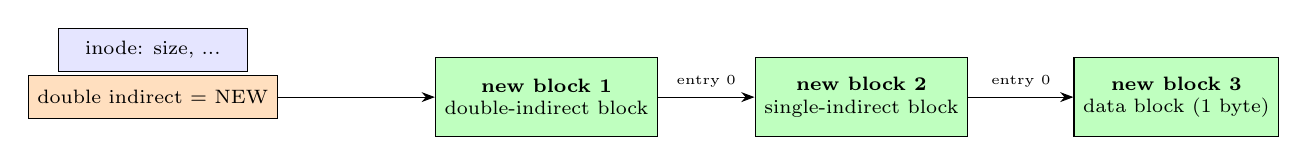
\begin{tikzpicture}[>=Stealth,font=\small]
\tikzstyle{c}=[draw,minimum height=0.55cm,minimum width=2.4cm,font=\scriptsize]
\node[c,fill=blue!10] (i) at (0,0) {inode: size, ...};
\node[c,fill=orange!25] (di) at (0,-0.6) {double indirect = NEW};
\node[draw,fill=green!25,minimum width=2.6cm,minimum height=1.0cm,font=\scriptsize,align=center] (b1) at (5,-0.6) {\textbf{new block 1}\\ double-indirect block};
\node[draw,fill=green!25,minimum width=2.6cm,minimum height=1.0cm,font=\scriptsize,align=center] (b2) at (9,-0.6) {\textbf{new block 2}\\ single-indirect block};
\node[draw,fill=green!25,minimum width=2.6cm,minimum height=1.0cm,font=\scriptsize,align=center] (b3) at (13,-0.6) {\textbf{new block 3}\\ data block (1 byte)};
\draw[->] (di.east) -- (b1.west); \draw[->] (b1.east) -- node[above,font=\tiny]{entry 0} (b2.west); \draw[->] (b2.east) -- node[above,font=\tiny]{entry 0} (b3.west);
\end{tikzpicture}
\end{document}
